\chapter{ANALISIS DAN PERANCANGAN}
\section{Analisis Sistem}
\par
Analisis sistem dapat diidentifikasikan sebagai penguraian dari suatu sistem informasi yang utuh kedalam bagian-bagian komponennya dengan maksud untuk mengidentifikasi dan mengevaluasi permasalahan, kesemptan, hambatan yang terjadi, dan kebutuhan yang diharapkan sehingga dapat menganalisis sistem yang berjalan. Pada bagian ini, hanya akan dibahas mengenai analisis pendaftaran online pemesan tiket bioskop melalui website CGV-blitz yang akan digambarkan dalam bentuk \textit{flowmap} dan \textit{Data Flow Diagram}.

\subsection{Analisis Sistem Berjalan}
\par
Gambaran tentang sistem yang saat ini sedang berjalan di \textit{website} CGV-blitz pada bagian proses pendaftaran online. Kami menganalisis fungsi bahasa pemrograman dan cara kerja sistem yang terdapat dalam proses tersebut. Analisis sistem ini bertujuan untuk mengetahui bagaiman cara kerja \textit{function} dan cara kerja sistem yang ada. 

\subsubsection{Analisis Prosedur (\textit{Flowmap})}
\textbf{A.	Analisis Sistem Pendaftaran Online}
\par
Analisis sistem yang sedang berjalan pada sistem pendaftaran online di \textit{website} CGV-blitz, bertujuan untuk mengetahui lebih jelas bagaimana cara kerja sistem dan \textit{function-function} yang tersedia. Perancangan analisis sistem yang sedang berjalan yang dilakukan berdasarkan urutan kejadian tersebut dapat dibuat diagram aliran ( \textit{flowmap}) prosedur sistem pendaftaran online, berikut gambar \ref{flowmapsistem} yang menjelaskan \textit{flowmap} sistem yang sedang berjalan di blitz : \\
\\
\\
\\

\begin{figure}[!htbp]
    \centering
    \includegraphics[scale=0.4]{gambar/flow1}
    \caption{\textit{Flowmap Sistem Yang Sedang Berjalan}}
    \label{flowmapsistem}
\end{figure}

\par
Berdasarkan \textit{flowmap} pada gambar\ref{flowmapsistem}, berikut adalah rincian aliran dari \textit{flowmap} tersebut
\begin{enumerate}
\item Start.
\item \textit{User} akan dialihkan ke menu utama.
\item Lalu pengguna akan menekan tombol \textit{"sign up"}, dan akan tertera form registrasi pada halaman tersebut.
\item Pengguna akan mengisi data diri sesuai data yang user miliki.
\item Sistem akan melakukan pengecekan apakah data tersebut sudah valid atau belum, jika belum pengguna akan dialihkan kembali ke menu pengisian data diri dan melakukan pengisian ulang, namun jika data sudah benar maka sistem akan memproses data tersebut.
\item Sistem akan mengirim validasi \textit{email} kepada pengguna.
\item Pengguna harus melakukan validasi kepada \textit{email}-nya, jika tidak maka pengguna harus kembali dan melakukan pengisian data diri ulang, namun jika \textit{email} sudah diverifikasi maka sistem akan kembali memroses verifikasi yang dilakukan oleh \textit{user}.
\item Sistem akan melakukan penyimpanan data \textit{user} kedalam \textit{database} sistem.
\item Sistem akan melakukan aktifasi akun \textit{user}
\item Akun \textit{user} telah aktif
\item Selesai
\end{enumerate}


\subsubsection{Analisis Dokumen Yang Digunakan}
\par
Analisis dokumen merupakan penjelasan mengenai dokumen-dokumen yang digunakan dalam sistem pendaftaran \textit{online}. Dalam tabel \ref{dokumen} merupakan analisa dokumen yang menjelaskan hal-hal yang akan dilakukan.
\\
\begin{table}[!htbp]
\captionsetup{singlelinecheck=off}
\caption{Dokumen Yang Digunakan}
\label{dokumen}
\begin{tabular}{|l|l|}
\hline
\textbf{Dibuat oleh} & CGV-BLITZ \\
\hline
\textbf{Dibuat untuk} & \textit{Konsumen} (Masyarakat)\\
\hline
\textbf{Isi} & list syarat pengajuan pendaftaran online akun CGV-BLITZ \\
\hline
\textbf{Frekuensi} & Dibuat sesuai dengan kebutuhan bersyarat \\ &    yang digunakan untuk melakukan pendaftaran online\\ 
\hline
\textbf{Tujuan} & Mempermudah proses membeli \\ & tiket bioskop online bagi masyarakat   \\
\hline
\end{tabular}
\end{table}


\subsection{Analisis Sistem Yang Akan Dibangun}
\par
Analisis kebutuhan yang dimaksud disini berupa analisis \textit{flowmap} mengenai sistem yang akan dibangun hanya meliputi sistem pendaftaran \textit{online} \textit{website} CGV-blitz.\\

\textbf{A.	Analisis sistem yang akan dibangun pada sistem pendaftaran \textit{online} }\\
\par
Didalam proses pendaftaran \textit{online} CGV-blitz ini, \textit{user} harus memasukkan beberapa data, dan hal itu kurang efektif waktu. Jadi kami menambahkan fitur melakukan registrasi menggunakan akun Gmail yang dimiliki \textit{user}.
\par
Berikut gambar\ref{flowmapbaru} yang menjelaskan tentang \textit{flowmap} yang akan dirancang.

\begin{figure}[!htbp]
    \centering
    \includegraphics[scale=0.6]{gambar/flow2}
    \caption{\textit{Rancangan Flowmap}}
    \label{flowmapbaru}
\end{figure}
\par
Berdasarkan gambar \textit{flowmap}\ref{flowmapbaru}, berikut adalah rincian aliran \textit{flowmap} yang akan dirancang nantinya
\begin{enumerate}
\item \textit{Start}.
\item Pengguna akan dialihkan ke menu utama.
\item Lalu pengguna akan menekan tombol \textit{"sign up"}, dan akan tertera form registrasi pada halaman tersebut.
\item Registrasi menggunakan akun Google+
\item Sistem akan melakukan pengecekan apakah data tersebut sudah valid atau belum, jika belum maka pengguna akan diarahkan kembali ke menu registrasi , namun jika data sudah benar maka sistem akan memproses data tersebut.
\item Data \textit{user} akan dimasukkan ke dalam \textit{database}, dan akun \textit{user} sudah aktif.
\item Selesai
\end{enumerate}

\subsubsection{Analisis Kebutuhan Aplikasi }
\par
Analisis kebutuhan aplikasi  merupakan suatu kebutuhan yang berhubungan dengan kebutuhan sistem yang akan dibuat. Dimana menjabarkan mengenai fungsi-fungsi yang dapat mendukung jalannya sistem, adapun kebutuhan aplikasi yang akan dibuat yaitu pengelolaan data terdiri dari 2 proses sesuai dengan urutan sebagai berikut:
\begin{enumerate}
\item	Pendaftaran Akun melalui Google+
\item	Aktifasi Akun
\end{enumerate}

\subsubsection{Analisis Kebutuhan Perangkat Lunak Dan Perangkat  Keras }
\par
Analisis kebutuhan perangkat lunak dilakukan untuk mengetahui spesifikasi kebutuhan untuk sistem. Spesifikasi kebutuhan melibatkan analisis perangkat keras/\textit{hardware}, analisis perangkat lunak/\textit{software}, analisis pengguna/\textit{User}. berikut tabel \ref{perangkatserver} ; \ref{perangkatclient} ; \ref{lunakserver} ; \ref{lunakclient} yang menjelaskan kebutuhan perangkat lunak dan perangkat keras yang nantinya akan digunakan.

\textbf{A.	Kebutuhan Perangkat Keras}

\begin{table}[!htbp]
\captionsetup{singlelinecheck=off}
\caption{Deskripsi perangkat \textit{server}}
\label{perangkatserver}
\begin{tabular}{|l|l|l|l|}
\hline
No & Nama Perangkat & Spesifikasi & Keterangan \\
\hline

1 &  \textit{Harddisk} & 500 GB  & Media untuk menyimpan \\
 & & & data aplikasi yang dibuat  \\
\hline

2 &  \textit{Memory} & 4 GB & \textit{Memory System} yang digunakan  \\
\hline

3 &  \textit{processor} & \textit{Intel® core™ i5-8250U  } &  Untuk kecepatan transfer data dari \\

 & & \textit{CPU @ 1.60GHz} &  sistem yang sangat bergantung \\
 
 & &\textit{(8 CPUs),~1.8Ghz} & pada kecepatan prosesor komputer \\
\hline

4 &  Infrastruktur Jaringan &    & Bisa dianalogikan sebagai \\     & & &  alur proses dari titik awal proses \\
& & & sampai pada akhir proses  \\

\hline
\end{tabular}
\end{table}


\begin{table}[!htbp]
\captionsetup{singlelinecheck=off}
\caption{Deskripsi perangkat \textit{client}}
\label{perangkatclient}
\begin{tabular}{|l|l|l|l|}
\hline
No & Nama Perangkat & Spesifikasi & Keterangan \\
\hline

1 &  \textit{Harddisk} & 250 GB  & Sebagai tempat penyimpanan data  \\
 & & & yang dibutuhkan,tetapi pada sisi\\
 & & & \textit{client} tidak diharuskan memiliki  \\
 & & & ketersediaan space yang besar \\
\hline

2 &  \textit{Memory} & 4 GB & Kecepatan \textit{client} dalam \\
 & & &  mengakses system ini  \\
\hline

3 &  \textit{processor} & \textit{Intel® core™ i5-8250U  } &  Untuk per halamanansi komputer \\

 & & \textit{CPU @ 1.60GHz} &  \\
 
 & &\textit{(8 CPUs),~1.8Ghz} & \\
\hline

4 &  Infrastruktur Jaringan &    & \textit{Server} dan \textit{Host} \\    
 & & &  alur proses dari titik awal proses \\
& & & sampai pada akhir proses  \\

\hline
\end{tabular}
\end{table}

\textbf{B.	Kebutuhan Perangkat Lunak}

\begin{table}[!htbp]
\captionsetup{singlelinecheck=off}
\caption{Deskripsi perangkat Lunak \textit{Server}}
\label{lunakserver}
\begin{tabular}{|l|l|l|l|}
\hline
No & \textit{Tools} & Fungsi & Keterangan \\
\hline

1 &  \textit{Windows 10} & Sistem Operasi  & -  \\

\hline

2 &  \textit{Xampp 1.7.3} & \textit{server} Basis Data & - \\
\hline

3 &  \textit{Photoshop CS} & desain antar muka & - \\
\hline

4 &  \textit{PHP,HTML,CSS} & \textit{Bahasa Program} & -  \\    
\hline

5 & \textit{sublime text} & software pendukung & - \\
\hline

6 & \textit{google chrome} & \textit{browser} & - \\
\hline
\end{tabular}
\end{table}


\begin{table}[!htbp]
\captionsetup{singlelinecheck=off}
\caption{Deskripsi Perangkat Lunak \textit{Client}}
\label{lunakclient}
\begin{tabular}{|l|l|l|l|}
\hline
No & \textit{Tools} & Fungsi & Keterangan \\
\hline

1 &  \textit{Windows 10} & Sistem Operasi  & -  \\

\hline

2 &  \textit{Xampp 1.7.3} & \textit{server} Basis Data & - \\
\hline

3 &  \textit{Photoshop CS} & desain antar muka & - \\
\hline

4 &  \textit{PHP,HTML,CSS} & \textit{Bahasa Program} & -  \\    
\hline

5 & \textit{sublime text} & software pendukung & - \\
\hline

6 & \textit{google chrome} & \textit{browser} & - \\
\hline
\end{tabular}
\end{table}

\textbf{C.	Analisis Pengguna/\textit{User}}
\par
Aplikasi yang akan dibuat ini hanya mencakup proses registrasi yang kelak nantinya akan digunakan oleh \textit{user} untuk melakukan pendaftaran akun. Yang diantaranya melibatkan Pengguna (masyarakat yang akan mendaftar pada akun CGV-BLITZ).

\section{Perancangan}
\subsection{\textit{Context Diagram}}
\par
\textit{Context diagram} berikut ini akan menggambarkan bagaimana proses keseluruhan dari sistem registrasi yang sedang berjalan di CGV blitz
pada gambar \ref{cd} merupakan \textit{context diagram} yang di analisis pada proses registrasi di aplikasi CGV Blitz

\begin{figure}[!htbp]
    \centering
    \includegraphics[scale=0.6]{gambar/cd.png}
    \caption{\textit{Context Diagram}}
    \label{cd}
\end{figure}

\subsection{\textit{Data Flow Diagram}}
\par
\textit{Data Flow Diagram} berikut akan memperinci pembahasan sistem registrasi yang sedang berjalan, yang nantinya dibagi menjadi beberapa proses. \textit{Data Flow Diagram} ini nantinya hanya mencakup \textit{DFD level} 0. 

\subsubsection{\textit{DFD Level} 0}
\par
Seperti dijelaskan sebelumnya, \textit{DFD level 0} ini merupakan penjabaran dari \textit{Context diagram} pada sistem aplikasi ini. \textit{DFD level 0} ini terdiri dari 2 (dua) proses sesuai dengan urutan sebagai berikut:
\begin{enumerate}
\item Proses registrasi
\item Aktifasi akun
\end{enumerate}

\par
Berikut pada gambar \ref{dfd0} merupakan \textit{DFD Level 0} sistem registrasi pada aplikasi CGV-blitz.

\begin{figure}[!htbp]
    \centering
    \includegraphics[scale=0.6]{gambar/dfd0.png}
    \caption{\textit{DFD0}}
    \label{dfd0}
\end{figure}
\par
Berdasarkan pada \ref{dfd0} \textit{DFD Level} 0 mencakup :
\begin{enumerate}
    \item Hanya terdapat satu entitas utama yaitu \textit{user}(pengguna aplikasi)
    \item Terdapat 2 proses utama yang berjalan pada sistem, yaitu proses registrasi, proses aktifasi akun. Dimana setiap proses ini mewakili beberapa proses dalam sistem dengan rincian sebagai berikut 
    \begin{enumerate}
        \item Proses registrasi mencakup proses registrasi data diri \textit{user} atau bisa menggunakan akun \textit{email} pengguna untuk melakukan registrasi.
        \item Aktifasi akun meliputi pengaktifan akun pengguna yang sudah melewati tahapan-tahapan registrasi.
    \end{enumerate}
\end{enumerate}

\subsection{Spesifikasi Proses \textit{(Process Specification)}}
\subsubsection{Spesifikasi Proses \textit{(Process Specification)} DFD Level 0}
\par
Berdasarkan pada tabel \ref{spesifikasidfd0}, akan menjelaskan spesifikasi dari table DFD level 0
\begin{table}[!htbp]
\captionsetup{singlelinecheck=off}
      \caption{\textit{tabel spesifikasi DFD level 0}}
    \label{spesifikasidfd0}
    \includegraphics[scale=0.6]{gambar/tabellogika.png}
\end{table}


\subsection{Kamus Alir Data\textit{(Data Flow Dictionary)}}
\par
Pada tabel \ref{Kamus Aliran Data} akan menjelaskan tentang kamus aliran data pada proses registrasi.

\begin{table}[!htbp]
\captionsetup{singlelinecheck=off}
\caption{Kamus Aliran Data}
\label{Kamus Aliran Data}
\begin{tabular}{|l|l|l|}
\hline
\textbf{No uji} & \textbf{Nama Alir Data} & \textbf{Keterangan}                  \\ \hline
1               & Pengisian Data          & /*Pengisian Data \textit{User} Dengan Gmail*/ \\ \hline

2               & Konfirmasi Akun               & /*Konfirmasi Akun \textit{User}*/             \\ \hline
3               & Konfirmasi Data               & /*Konfirmasi Data \textit{User}*/             \\ \hline

4               & Aktifasi Akun           & /*Pengaktifan Akun \textit{User}*/          \\ \hline
\end{tabular}
\end{table}
\subsection{Perancangan \textit{Database}}
\subsubsection{\textit{Conceptual Data Model}}
\par
Pada gambar \ref{cdm} adalah perancangan \textit{database} registrasi pada aplikasi CGV-blitz dalam benduk \textit{Conceptual Data Model} (CDM).


\begin{figure}[!htbp]
    \centering
    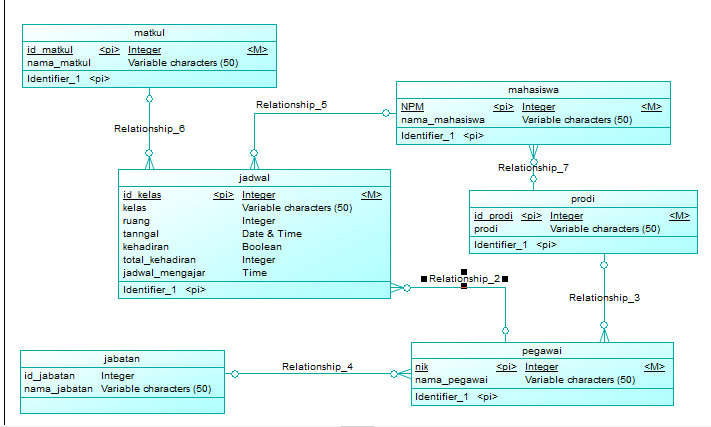
\includegraphics[scale=0.6]{gambar/CDM}
    \caption{\textit{CDM}}
    \label{cdm}
\end{figure}

\subsubsection{\textit{Physical Data Model}}
\par
Pada gambar \ref{pdm} merupakan perancangan \textit{database} registrasi pada aplikasi CGV-blitz dalam benduk \textit{Physical Data Model} (PDM)


\begin{figure}[!htbp]
    \centering
    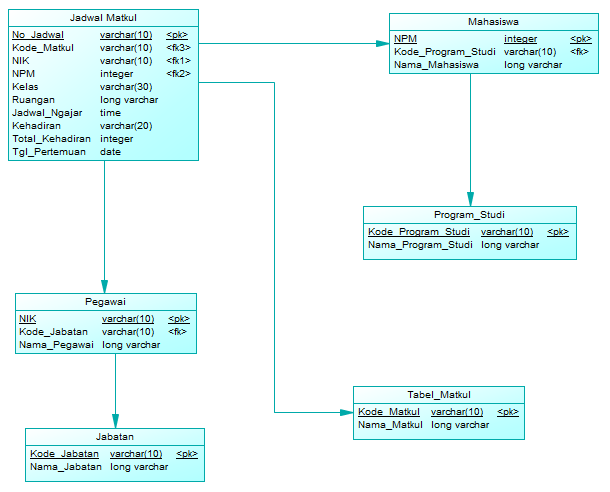
\includegraphics[scale=0.6]{gambar/PDM}
    \caption{\textit{PDM}}
    \label{pdm}
\end{figure}

\subsubsection{\textit{Kamus Data Tabel(Database)}}
\par
Pada tabel \ref{kamusdata} ; \ref{kamusdata2} ; \ref{kamusdata3} ; \ref{kamusdata4}, menjelaskan tentang kamus data tabel \textit{database}.

\begin{table}[!htbp]
\captionsetup{singlelinecheck=off}
\caption{\textit{User}}
\label{kamusdata}
\begin{tabular}{|l|l|l|l|l|}
\hline
No & \textit{Field} & \textit{Type} & Panjang & keterangan \\
\hline

1 &  \textit{Name} & \textit{Variable Character}  & 50 & -  \\

\hline

2 &  \textit{Birthdate} & \textit{VarChar}  & 35 & tanggal lahir \\
\hline

3 &  \textit{Phone Number} & \textit{Integer} &  & nomor telpon  \\
\hline

4 &  \textit{email address} & \textit{VarChar} & 50 & \textit{email user}  \\    
\hline

5 & \textit{Password} & \textit{VarChar} & 50 &  \\
\hline

6 & \textit{Pin} & \textit{integer} &  & \\
\hline

7 & \textit{CGV card} & \textit{integer} & &\\
\hline 
\end{tabular}
\end{table}


\begin{table}[!htbp]
\captionsetup{singlelinecheck=off}
\caption{\textit{Captcha}}
\label{kamusdata2}
\begin{tabular}{|l|l|l|l|l|}
\hline
No & \textit{Field} & \textit{Type} & Panjang & keterangan \\
\hline

1 &  \textit{Captcha ID} & \textit{Integer}  &  &   \\

\hline

2 &  \textit{Captcha number} & \textit{Integer}  &  & Kode \textit{Captcha} \\
\hline

\end{tabular}
\end{table}

\begin{table}[!htbp]
\captionsetup{singlelinecheck=off}
\caption{\textit{City}}
\label{kamusdata3}
\begin{tabular}{|l|l|l|l|l|}
\hline
No & \textit{Field} & \textit{Type} & Panjang & Keterangan \\
\hline

1 &  \textit{City ID} & \textit{Integer}  &  &   \\

\hline

2 &  \textit{City name} & \textit{Integer}  &  & Nama kota \\
\hline

\end{tabular}
\end{table}


\begin{table}[!htbp]
\captionsetup{singlelinecheck=off}
\caption{\textit{Cinema}}
\label{kamusdata4}
\begin{tabular}{|l|l|l|l|l|}
\hline
No & \textit{Field} & \textit{Type} & Panjang & keterangan \\
\hline

1 &  \textit{Cinema ID} & \textit{Integer}  &  &   \\

\hline

2 &  \textit{Cinema name} & \textit{VarChar} & 35 & Nama Bioskop \\
\hline

\end{tabular}
\end{table}


\subsection{Struktur Menu}
\par
Berikut pada gambar \ref{struktur}, menggambarkan struktur menu yang ada di aplikasi CGV-blitz.
\begin{figure}[!htbp]
    \centering
    \includegraphics[scale=0.5]{gambar/STRUKTUR}
    \caption{\textit{struktur menu}}
    \label{struktur}
\end{figure}

\par
Berdasarkan pada gambar \ref{struktur}, laporan ini hanya akan membahas bagaimana proses registrasi blitz berjalan. Didalam bagan ini proses registrasi ditandai dengan model subproses, yang bentuknya seperti pada gambar \ref{sub} berikut yang menggambarkan bagaimana bentuk subproses itu sendiri.

\begin{figure}[!htbp]
    \centering
    \includegraphics[scale=0.5]{gambar/sub}
    \caption{\textit{sub proses}}
    \label{sub}
\end{figure}
\subsection{Perancangan Antar Muka}
\par
Berikut adalah rincian \textit{coding} perancangan antar muka yang akan dibangun.

\subsubsection{\textit{Index}}

\begin{figure}[!htbp]
    \centering
    \includegraphics[scale=0.5]{gambar/index}
    \caption{\textit{Fungsi Index}}
    \label{index}
\end{figure}


\par
Berdasarkan pada gambar \ref{index} , merupakan fungsi yang nantinya akan menampilkan tampilan registrasi menggunakan Google+. dengan rincian sebagai berikut.

\begin{figure}[!htbp]
    \centering
    \includegraphics[scale=0.5]{gambar/indexphp}
    \caption{\textit{Fungsi PHP Pada Index}}
    \label{indexphp}
\end{figure}

\par 
Berdesarkan pada gambar \ref{indexphp} , fungsi \textit{PHP} disini digunakan untuk menghubungkan fungsi \textit{coding} pada halaman lain, dan ditempatkan sebelum \textit{coding HTML}. Fungsi dari \textit{coding} tersebut dapat dijabarkan sebagai berikut.
\\
\\
\\

\begin{enumerate}
\item \textit{"require once"} : Membutuhkan suatu file agar fungsi tersebut bisa berjalan, apabila file tersebut tidak ditemukan maka fungsi selanjutnya tidak akan dijalankan.
\item \textit{"if"} : Fungsi untuk permisalan
\item \textit{"isset"} : Untuk meng-\textit{"set"} suatu variable yang nantinya akan dijalan kan, jika variable berhasil di \textit{set} maka akan mengembalikan nilai \textit{TRUE}, jika sebaliknya maka akan mengembalikan nilai \textit{FALSE}.
\item \textit{"session" }: Untuk mengingat data yang sudah diinputkan oleh \textit{user}.
\item \textit{"header" }: Untuk mengarah ke fungsi \textit{coding} yang lain.
\item \textit{"exit" }: Untuk keluar dari fungsi tersebut.
\item \textit{"LoginURL = client-createAuthUrl()" }: Variabel dari \textit{LoginURL} memiliki nilai berupa \textit{variable client} yang mengarah ke \textit{method createAuthUrl()}.
\end{enumerate}


\par 
Setelah memasukkan fungsi \textit{PHP} selanjutnya diikuti oleh \textit{coding HTML} seperti pada gambar \ref{indexhtml} berikut.

\begin{figure}[!htbp]
    \centering
    \includegraphics[scale=0.5]{gambar/indexhtml}
    \caption{\textit{HTML Pada Index}}
    \label{indexhtml}
\end{figure}
\par 
\textit{Coding HTML} disini berfungsi untuk membuat tampilan \textit{user interface}. berikut penjabaran \textit{fungsi coding HTML}.
\begin{enumerate}
\item \textit{"html"} : Untuk memulai fungsi \textit{HTML}
\item \textit{"head"} : Header pada \textit{HTML}
\item \textit{"title"} : Untuk menempatkan judul pada \textit{coding HTML}
\item \textit{"body"} : Untuk "isi" yang ada pada \textit{HTML}
\item \textit{"input type....login with google"} : Untuk membuat tombol login yang nantinya jika ditekan akan mengarah ke tampilan \textit{ log in google}
\end{enumerate}

\subsubsection{\textit{Config}}
\begin{figure}[!htbp]
    \centering
    \includegraphics[scale=0.5]{gambar/config}
    \caption{\textit{Fungsi PHP Pada Config}}
    \label{config}
\end{figure}
\par 
Berdasarkan pada gambar \ref{config}, fungsi config ini memegang peran penting dalam berjalannya rencangan aplikasi ini, karena file config ini mengandung fungsi yang menghubungkan aplikasi kepada Google+ \textit{API}. Seperti \textit{coding} yang tertera berikut
\par 
\textit{GoogleAPI/vendor/autoload.php}
\par 
Pada coding tersebut kita memanggil semua fungsi yang dibutuhkan untuk menyambungkan aplikasi kepada google+ \textit{API}.

\subsubsection{\textit{Callback}}
\begin{figure}[!htbp]
    \centering
    \includegraphics[scale=0.5]{gambar/callback}
    \caption{\textit{Fungsi PHP Pada Callback}}
    \label{callback}
\end{figure}
\par 
Berdasarkan pada gambar \ref{callback}, fungsi file \textit{callback} disini adalah untuk melakukan pengecekan apakah akun \textit{user} sudah pernah diregistrasikan atau belum, berikut penjelasan logika dari file \textit{callback} tersebut
\\
\\
\\
\begin{enumerate}
\item \textit{"if"} (jika) akun tersebut sebelumnya sudah pernah diregistrasi, maka akan langsung dialihkan ke bagian \textit{login.php}
\item \textit{"if else"} (jika tidak) akun tersebut akan didaftarkan, jika berhasil didaftarkan makan akan langsung menuju ke bagian \textit{login.php}
\item \textit{"else"} (tidak) jika proses registrasi gagal maka akan dialihkan ke bagian \textit{index.php}
\end{enumerate}
\par
Dalam fungsi ini juga digunakan \textit{method}get(), \textit{method} ini digunakan untuk mengambil info data pada akun \textit{user}, dalam fungsi coding pada gambar \ref{callback} data yang diambil berupa \textit{uid,email},dan juga \textit{gender}. Dan disimpan menggunakan fungsi \textit{session}.


\subsubsection{\textit{Login}}
\begin{figure}[!htbp]
    \centering
    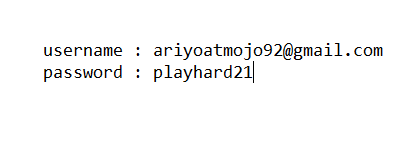
\includegraphics[scale=0.5]{gambar/login}
    \caption{\textit{Fungsi Pada Login}}
    \label{login}
\end{figure}
\par 
Berdasarkan pada gambar \ref{login}, fungsi ini akan menampilkan informasi yang sebelumnya telah disimpan dan dijelaskan pada gambar \ref{callback}. tedapat 2 fungsi pada \textit{coding}-an ini, pertama adalah \textit{coding fungsi PHP} yang diletakkan sebelum fungsi \textit{HTML}, dan \textit{coding HTML} yang digunakan sebagai fungsi untuk \textit{user interface}. Berikut adalah penjabaran \textit{fungsi-fungsi} tersebut.
\begin{enumerate}
\item 
\begin{figure}[!htbp]
    \centering
    \includegraphics[scale=0.5]{gambar/loginphp}
    \caption{\textit{Fungsi \textit{PHP} Pada \textit{Login}}}
    \label{loginphp}
\end{figure}
\par 
Pada gambar \ref{loginphp}, fungsi yang digunakan adalah untuk melakukan pengecekan terhadap \textit{session} yang sudah di set, jika tidak ditemukan maka \textit{user} akan dialihkan kembali ke \textit{login.php} .

\item
\begin{figure}[!htbp]
    \centering
    \includegraphics[scale=0.5]{gambar/loginhtml}
    \caption{\textit{Fungsi \textit{HTML} Pada \textit{Login}}}
    \label{loginhtml}
\end{figure}
\par 
Fungsi \textit{HTML} yang digunakan disini untuk menampilkan hasil tampilan data yang sudah disimpan berdasarkan gambar \ref{callback}. Penjabaran fungsi tambahan yang ada pada gambar \ref{loginhtml} adalah sebagai berikut.
\\
\begin{enumerate}
\item \textit{"tr"} : Untuk membuat baris tabel.
\item \textit{"td"} : Untuk membuat data tabel.
\item \textit{"echo session (gender/email/uid)"} : Untuk memanggil data yang disimpan di \textit{session}.
\end{enumerate}
\end{enumerate}


\subsubsection{\textit{Dbconfig}}
\begin{figure}[!htbp]
    \centering
    \includegraphics[scale=0.5]{gambar/db}
    \caption{\textit{Fungsi \textit{PHP} Pada \textit{Dbconfig}}}
    \label{dbconfig}
\end{figure}
\par 
Berdasarkan pada gambar \ref{dbconfig}, fungsi dari codingan \textit{PHP} di file \textit{Dbconfig} ini adalah untuk mengkoneksikan aplikasi rancangan kita ke database. Perincian fungsi php tersebut adalah sebagai berikut
\begin{enumerate}
\item \textit{"define('DB SERVER, localhost').....('DB DATABASE','google')"} : Untuk membedakan \textit{database localhost}, beserta \textit{input username,password}, dan nama tabel
\item \textit{"mysql connect"} : Untuk menenghubungkan \textit{database} ke \textit{localhost}, beserta \textit{input username}, dan \textit{password}. Dan jika gagal maka error
\item \textit{"mysql select db"} : Untuk Menentukan tabel mana yang akan digunakan, jika gagal maka error.
\end{enumerate}


\subsubsection{\textit{Function}}
\begin{figure}[!htbp]
    \centering
    \includegraphics[scale=0.5]{gambar/fungsi}
    \caption{\textit{Fungsi \textit{PHP} Pada \textit{Function}}}
    \label{fungsi}
\end{figure}
\par
Mengacu pada gambar \ref{fungsi}, fungsi \textit{file function} disini adalah sebagai sambungan dari pengkoneksian \textit{database}, dengan perincian fungsi sebagai berikut
\\
\\
\\
\\
\par
Fungi \textit{SQL}
\begin{enumerate}
\item \textit{Select} : Memilih nama tabel yang akan digunakan.
\item \textit{Insert} : Memasukkan nilai kedalam tabel yang akan dipilih.
\item \textit{Update} : Memperbarui data terbaru yang diinput.
\end{enumerate}
\par 
Fungsi Menyeluruh
\begin{enumerate}
\item \textit{if}(jika) data yang diinputkan sebelumnya tidak ada/kosong, maka akan menginputkan data baru ke dalam tabel google
\item \textit{else}(lainnya) mengupdate data lama yang sebelumnya disimpan didalam \textit{database}.
\end{enumerate}


\subsubsection{Pembuatan \textit{Database}}
\begin{figure}[!htbp]
    \centering
    \includegraphics[scale=0.5]{gambar/buat}
    \caption{\textit{Pembuatan \textit{Database}}}
    \label{pembuatandb}
\end{figure}
\par 
Berdasarkan pada gambar \ref{pembuatandb}, \textit{database} dapat dijabarkan pengertiannya sebagai berikut
\begin{enumerate}
	\item \textit{"id"} : Memiliki tipe data \textit{\textbf{INTEGER}} dan bertipe \textit{\textbf{NOT NULL}}
	serta akan menambah seiring adanya data baru \textit{(AUTO INCREMENT)}, dan berstatus \textit{PRIMARY KEY} yang memiliki arti bahwa id ini merupakan pembeda dari atribut pada tabel-tabel yang lain
	\item \textit{"UID"} : Memiliki tipe data \textit{\textbf{VARCHAR}} yang memiliki panjang sepanjang 30 dan bertipe \textit{\textbf{NOT NULL}}
	\item \textit{"email"} : Memiliki tipe data \textit{\textbf{VARCHAR}} yang memiliki panjang sepanjang 50 dan bertipe \textit{\textbf{NOT NULL}}
	\item \textit{"gender"} : Memiliki tipe data \textit{\textbf{VARCHAR}} yang memiliki panjang sepanjang 20 dan bertipe \textit{\textbf{NOT NULL}}
\end{enumerate}


\par
Berdesarkan data diatas, kata yang bercetak tebal memiliki arti sebagai berikut.
\begin{enumerate}
\item \textit{INTEGER} : Data yang dimasukkan hanya berupa angka tidak bisa yang lain.
\item \textit{VARCHAR (Variable Character)} : Data yang dimasukkan berupa \textit{character}.
\item \textit{NOT NULL} : Data yang akan diisi tidak boleh kosong.
\end{enumerate}